\section{SimSite3D::hbond\_\-ideal\_\-pt\_\-base Class Reference}
\label{classSimSite3D_1_1hbond__ideal__pt__base}\index{SimSite3D::hbond_ideal_pt_base@{SimSite3D::hbond\_\-ideal\_\-pt\_\-base}}
An \char`\"{}ideal\char`\"{} hbond point base class.  


{\tt \#include $<$hbond\_\-points.H$>$}

Inheritance diagram for SimSite3D::hbond\_\-ideal\_\-pt\_\-base::\begin{figure}[H]
\begin{center}
\leavevmode
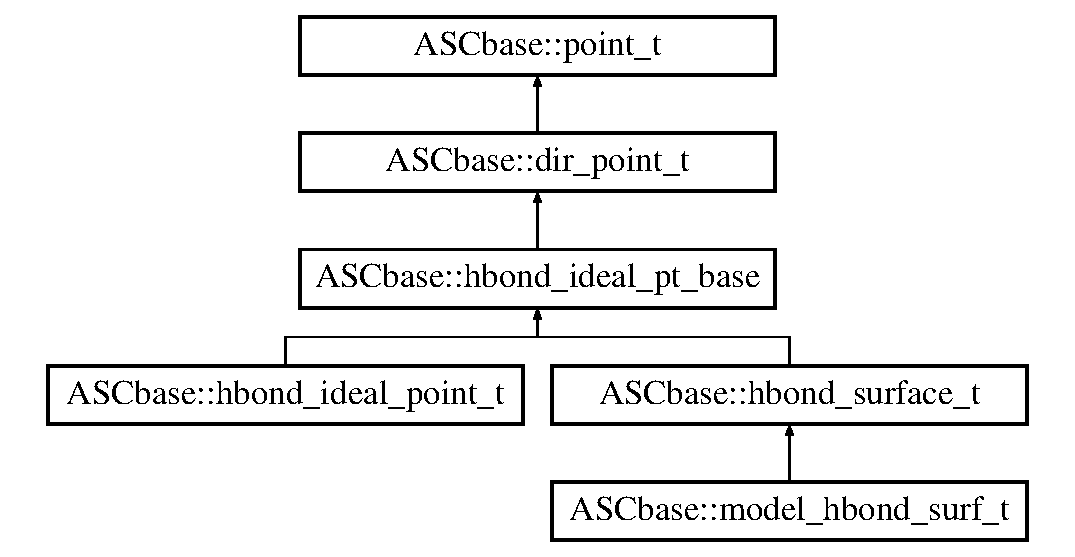
\includegraphics[height=5cm]{classSimSite3D_1_1hbond__ideal__pt__base}
\end{center}
\end{figure}
\subsection*{Public Member Functions}
\begin{CompactItemize}
\item 
\textbf{hbond\_\-ideal\_\-pt\_\-base} (alloc\_\-t a=ALLOC\_\-POSITION)\label{classSimSite3D_1_1hbond__ideal__pt__base_6c727a2312275eeca47a7a36b27ff531}

\item 
\textbf{hbond\_\-ideal\_\-pt\_\-base} (const atom\_\-vci hbond\_\-atom, const atom\_\-vci C\_\-nbr\_\-atom, const atom\_\-vci second\_\-nbr\_\-atom, const \bf{Bounding\-Volume} \&site\_\-vol, const int cap\_\-number, const bool include\_\-metals=false, const alloc\_\-t a=ALLOC\_\-POSITION)\label{classSimSite3D_1_1hbond__ideal__pt__base_8c6aebede051225c5d7732dff3c9de61}

\item 
\textbf{hbond\_\-ideal\_\-pt\_\-base} (const \bf{hbond\_\-ideal\_\-pt\_\-base} \&p)\label{classSimSite3D_1_1hbond__ideal__pt__base_6b1afae556e880d14099bdca58304d46}

\item 
const \bf{hbond\_\-ideal\_\-pt\_\-base} \& \textbf{operator=} (const \bf{hbond\_\-ideal\_\-pt\_\-base} \&p)\label{classSimSite3D_1_1hbond__ideal__pt__base_a8a595d97addfd2dc71a74230a022dec}

\item 
const \bf{SimSite3D::atom\_\-t} \& \textbf{\_\-\_\-get\_\-atom} () const \label{classSimSite3D_1_1hbond__ideal__pt__base_4ad13839630fecd1c9d561e081b7b18e}

\item 
const \bf{SimSite3D::atom\_\-t} \& \textbf{\_\-\_\-get\_\-carbon\_\-nbr} () const \label{classSimSite3D_1_1hbond__ideal__pt__base_1e47efb94434d32735034ade4ee4a7fe}

\end{CompactItemize}
\subsection*{Static Public Member Functions}
\begin{CompactItemize}
\item 
static bool \textbf{cmp} (const \bf{hbond\_\-ideal\_\-pt\_\-base} \&A, const \bf{hbond\_\-ideal\_\-pt\_\-base} \&B)\label{classSimSite3D_1_1hbond__ideal__pt__base_6d6b4ad446addecc3079229713313731}

\end{CompactItemize}
\subsection*{Public Attributes}
\begin{CompactItemize}
\item 
uint \bf{pt\_\-num}\label{classSimSite3D_1_1hbond__ideal__pt__base_a6829823658e609726d64d46f05a53c4}

\begin{CompactList}\small\item\em Number given to the ideal point. \item\end{CompactList}\item 
interaction\-Type \bf{act\_\-type}\label{classSimSite3D_1_1hbond__ideal__pt__base_2b226c040314c92bf0e9d0e647f66897}

\begin{CompactList}\small\item\em Interaction type of the points. \item\end{CompactList}\item 
atom\_\-vci \bf{atom}\label{classSimSite3D_1_1hbond__ideal__pt__base_c69850f24c46ac0c32143cf6f3ac2c91}

\begin{CompactList}\small\item\em Protein heavy atom giving rise to the points. \item\end{CompactList}\item 
atom\_\-vci \bf{carbon\_\-nbr}\label{classSimSite3D_1_1hbond__ideal__pt__base_7155ffb9e0c06bc4267fb4ee28b9d212}

\begin{CompactList}\small\item\em Carbon atom used to define the acceptor/donor plane. \item\end{CompactList}\item 
atom\_\-vci \bf{second\_\-nbr}\label{classSimSite3D_1_1hbond__ideal__pt__base_733afddb617c0b55f4887e963d954848}

\begin{CompactList}\small\item\em Third atom used to define the plane. \item\end{CompactList}\end{CompactItemize}
\subsection*{Private Member Functions}
\begin{CompactItemize}
\item 
void \textbf{do\_\-copy} (const \bf{hbond\_\-ideal\_\-pt\_\-base} \&p)\label{classSimSite3D_1_1hbond__ideal__pt__base_ea14650cc4989d996bb228f2d68e2cee}

\end{CompactItemize}


\subsection{Detailed Description}
An \char`\"{}ideal\char`\"{} hbond point base class. 



The documentation for this class was generated from the following file:\begin{CompactItemize}
\item 
hbond\_\-points.H\end{CompactItemize}
